%!TEX root = kudzai_thesis.tex
%%%%%%%%%%%%%%%%%%%%%%%%%%%%%%%%%%%%%%%%%%%%%%%%%%%%%%%%%%%%%%%%%%%%%%%
\chapter{Basics of Sentiment analysis}\label{ch:THEORY}

\begin{summary}
  Please provide specifics of the CONTENT.
  
  only after the chapter is finished!
\end{summary}


There are two approaches to sentiment analysis: lexicon-based and machine learning-based. 
%
Machine learning as the name suggests requires the model to be trained, lexicon based consists of a set of rules and doesn’t require prior training, a third method although not used very often is a hybrid method that combines both lexicon and machine learning approaches, generally it yields better results than either method individually.
%
In table~\ref{tab:sent_analysis_approaches} will summarize the differences between the two approaches. 
 
\begin{table}[h]
  \centering
  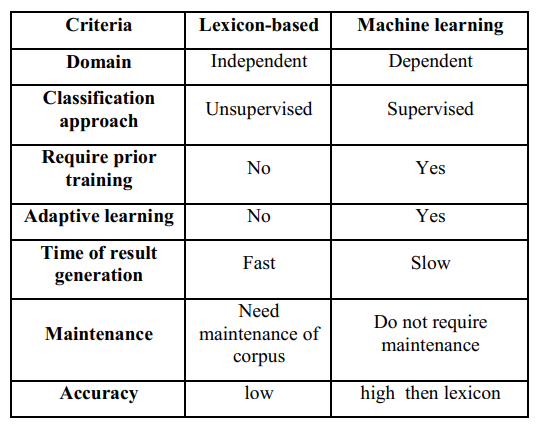
\includegraphics[width=0.5\linewidth]{images/lex_vs_ml.png}
  \caption{Comparison between lexicon and machine learning}
  \label{tab:sent_analysis_approaches}
\end{table}

Sentiment analysis seeks to classify text as either positive or negative or neutral, using methods in Natural language processing (NLP). The common approach implemented involves statistical analysis and machine learning methods. However spoken and written language is ambiguous but fuzzy systems are well suited to deal with ambiguity. The proposed system will be a hybrid system it will use both machine learning approach as well as lexicon-based approach to classify the sentences polarity, the system will tokenize any given document into chunks, and feed each chunk into the classifier. The document is tokenized based on disjunctive words such as BUT, and OR and grammatical structures e.g. a period or a comma. The results of each individual sentence will be passed into the fuzzy classifier and an emotion will be detected.	

\clearpage




\section{
LSTM(TensorFlow)
}
Long short-term memory (LSTM) is an artificial recurrent neural network (RNN) architecture used in the field of deep learning. (LSTM) networks are an extension for recurrent neural networks, which basically extends their memory. Therefore, it is well suited to learn from important experiences that have very long-time lags in between. 
The memory of an LSTM is a gated cell, the gated cell decides to retain or to delete information by opening or closing its gate respectively, it decides this according to the relevance it assigns to the information. Relevance of information depends on the weights assigned to the information which are learned by the algorithm during training. 
LSTM have 3 gates, the input gate determines when to let new information in, the forget gate determines what information will be retain both these gates will affect the output gate. \\ \\
Below is a diagram of the LSTM 

\begin{figure}[h]
    \centering
    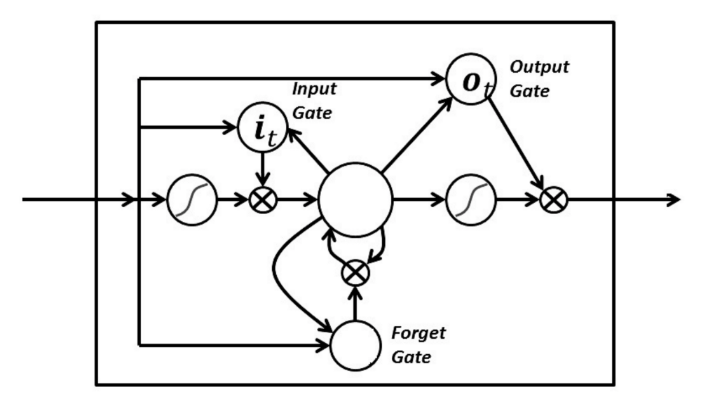
\includegraphics[width=0.5\linewidth]{images/lstm.png}
    \caption{Diagram of LSTM}
\end{figure}


\subsection{Lexicon (VaderSentiment)}
An emoticon, short for "emotion icon", also known simply as an emote, is a pictorial representation of a facial expression using characters usually punctuation marks, numbers and letters to express a person's feelings or mood, or as a time-saving method rather than to type out a whole word, an emoticon can be used to convey the writer's feelings or intended tone. \\ \\
A lexicon is a collection of information about the words of a language about the lexical categories to which they belong. Lexicon based sentiment analysis makes use of labeled text this is very useful in detecting sentiment by emoticons. I will use a python library called VaderSentiment.\\ \\
VADER (Valence Aware Dictionary and sEntiment Reasoner) is a lexicon and rule-based sentiment analysis tool that is specifically attuned to sentiments expressed in social media. VADER uses a combination of A sentiment lexicon is a list of lexical features (e.g., words) which are generally labelled according to their semantic orientation as either positive or negative. In addition to this I will also add a list of commonly used acronyms that express sentiment such as OMG, SMH, LOL, ROTF \\
Some key features of Vader sentiment are: -

\begin{enumerate}

\item	
Punctuation: The use of an exclamation mark(!), increases the magnitude of the intensity without modifying the semantic orientation. For example, “The food here is good!” is more intense than “The food here is good.” and an increase in the number of (!), increases the magnitude accordingly.
    
\item
Capitalization: Using upper case letters to emphasize a sentiment-relevant word in the presence of other non-capitalized words, increases the magnitude of the sentiment intensity. For example, “The food here is GREAT!” conveys more intensity than “The food here is great!”
\item 
Degree modifiers: Also called intensifiers, they impact the sentiment intensity by either increasing or decreasing the intensity. For example, “The service here is extremely good” is more intense than “The service here is good”, whereas “The service here is marginally good” reduces the intensity.
\item 
Conjunctions: Use of conjunctions like “but” signals a shift in sentiment polarity, with the sentiment of the text following the conjunction being dominant. “The food here is great, but the service is horrible” has mixed sentiment, with the latter half dictating the overall rating.
\item 
Preceding Tri-gram: By examining the tri-gram preceding a sentiment-laden lexical feature, we catch nearly 90\% of cases where negation flips the polarity of the text. A negated sentence would be “The food here isn’t really all that great”.
\end{enumerate}

\clearpage
\subsection{Fuzzy Logic (emotion classification)}
Fuzzy logic is a form of many-valued logic in which the truth values of variables may be any real number between 0 and 1 inclusive. It is employed to handle the concept of partial truth, where the truth value may range between completely true and completely false. It is an approach to computing based on "degrees of truth" often called the degree of membership, rather than the usual "true or false" (1 or 0) Boolean logic on which the modern computer is based.

\begin{figure}[h]
    \centering
    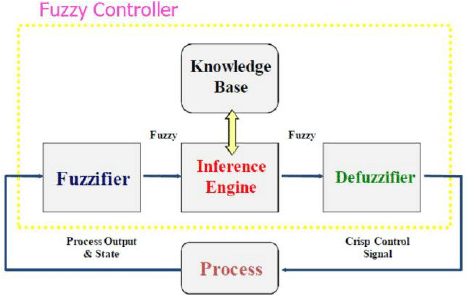
\includegraphics[width=0.5\linewidth]{images/fuzzy_logic.png}
    \caption{Block Diagram of fuzzy inference system}
    \label{fig:my_label}
\end{figure}

\clearpage
\subsection{Subjectivity and Objectivity (TextBlob)}
Being able to detect subjectivity and objectivity is an important part of sentiment analysis, because it can tell us more about the authors emotions. I will use a python library called TextBlob to detect the degree of subjectivity and the degree of objectivity, these results will be added to the fuzzy emotion detection. The degree of subjectivity and objectivity will affect the emotion classification. That is to say is the author being sarcastic or is the author being impartial or is the author expressing some significant sentiment towards a topic.

\clearpage

\subsection{Confusion matrix}
A confusion matrix is used in machine learning to determine the performance of a classification algorithm. It is a tabular form than compares test data for which its true values are known. I will use the confusion matrix to compare the performance of my own system against that of the Naïve Bayes classifier which is known to often perform well in sentiment analysis.
For example, if there are two possible predicted classes: "yes" and "no". If we were predicting the presence of a disease, for example, "yes" would mean they have the disease, and "no" would mean they don't have the disease.
 \begin{itemize}
    
\item 
true positives (TP): This is when we have given a correct positive prediction

\item
true negatives (TN): This is when we have given a correct negative prediction.

\item 
false positives (FP): This is when we have predicted yes, but the true value is no

\item 
false negatives (FN): This is when we have predicted no, but the true value is yes
 
\end{itemize}

\begin{figure}[h]
    \centering
    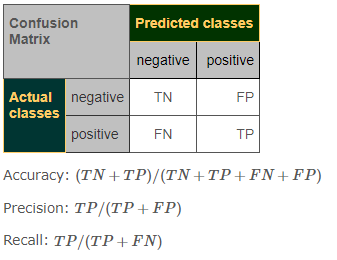
\includegraphics{images/confusion_matrix.png}
    \caption{Confusion matrix}
\end{figure}

  The above table shows how to determine the accuracy of the prediction using a confusion matrix. However, there are problems with accuracy. It assumes equal costs for both kinds of errors that is to say it assumes that we have an equal number of positives and negatives. A 99\% accuracy can either be excellent, good, mediocre, poor or terrible depending upon the problem
  
\section{Expected Results and analysis}

\subsection{Implementing (LSTM)}

I will make use of an open source Machine Learning library by Google brain team called TensorFlow. The aim of the (LSTM) model is to take a sentence, paragraph, document, or any piece of natural language, and determine whether that text's emotional tone is positive, negative or neutral. LSTM makes use of word vectors I will describe word vectors in brief.\\ \\
Word vectors are actual numeric vectors used to represent a word in a given context. word vectors use one hot encoding to represent the position of the word of interest in a given sequence of words and a zero in all other places. Word vectors do not capture the meaning of the word but only the potential relationships it has with its contextual neighbors. The advantage of representing words as vectors is that we can use mathematical functions on the vectors that represent the words, we can do addition, subtraction, multiplication and even compute the distance between two vectors.\\ \\
The below diagram shows how a vector for adore is closer to the vector for love than it is to the vector for baseball. This is because they both have similar meanings and can be found in similar contexts.


\begin{figure}[h]
    \centering
    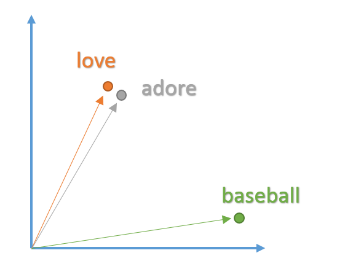
\includegraphics{images/word_vec_1.png}
    \caption{word vector}
\end{figure}



\subsection{Implementing subjectivity/objectivity detection using VaderSentiment and TextBlob}
TextBlob and VaderSentiment are both python libraries for natural language processing build on top on NLTK, they can do sentiment analysis and some additional functions such as part of speech tagging (POS), part of speech tagging is a feature that can identify nouns and pronouns and adjectives in a sentence. I will begin by training the models on a text file of positive and negative movie reviews.\\ \\
After training the models, I will create a TextBlob object and pass the sentence that I want to classify into the constructor of the TextBlob object, with the textblob object initialized I can now call some functions on the object, the “.sentiment member function” will show the degree of positive, negative, neutral and also the subjectivity of the sentence. The polarity of the given sentence is ranges from +1 to -1 with 0 being neutral, subjectivity is measured from 0 to 1 with 0 being objective and 1 being subjective.



With VaderSentiment I will create  a SentimentIntensityAnalyser() object and call the .polarity\_scores() member function and pass the string into the function, the object will return the polarity scores positive(between 0 and 1), negative(between 0 and 1), neutral(between 0 and 1) and also compound(between 0 and 1). The compound score is computed as the following: according to the VaderSentiment website. The compound score is computed by summing the valence scores of each word in the lexicon, adjusted according to the rules, and then normalized to be between -1(most extreme negative) and +1(most extreme positive). This is the most useful metric if you want a single unidimensional measure of sentiment for a given sentence. 


\subsection{Implementing fuzzy logic classifier}

The human language is complex. Teaching a machine to analyze the various grammatical nuances, cultural variations, slang and misspellings that occur in online mentions is a difficult process. Teaching a machine to understand how context can affect tone is even more difficult. Humans are fairly intuitive when it comes to interpreting the tone of a piece of writing. But with fuzzy logic a machine can have an imprecise input and produce a precise output, this is achieved by using membership functions and evaluating the degree of membership of each category then taking the highest value to give the precise classification.\\ \\

I will classify the emotion from a tweet using the following categories:



\textbf{Happy, Sad, Angry, Disappointed, Surprised, Proud, Scared}
\begin{itemize}
\item
Step 1: tokenize the document into sentences, tokenization will be done based on punctuation i.e. using comma or period and disjunctive words like “but”, “or”.
\item
Step 2: pass each part of the sentence into the LSTM, VaderSentiment, TextBlob analyzer.
\item
Step 3: determine the degree of membership of each of the sentence parts.
\item
Step 4: aggregate the scores to classify the document into the emotion group.

\end{itemize}







%%%%%%%%%%%%%%%%%%%%%%%%%%%%%%%%%%%%%%%%%%%%%%%%%%%%%%%%%%%%%%%%%%%%%%%
\section{Linear discriminant}\label{sec:THEORY:linear}

There is often equation:
\begin{equation}
	f: \Omega_x \rightarrow {\mathbb{R}}
	\quad\text{ such that }
	\quad f(x)
	\begin{cases}
		<0 & \forall x\in Neg \\
		\geq 0 & \forall x\in Poz
	\end{cases}
	\label{eq:diszkr:fugg}
\end{equation}



If an equation is not very important, one can use the \$\$ notation...

$$D_k(x)=\tilde{x}^T\alpha_k=\alpha_k^T\tilde{x},$$

